\documentclass[a4paper,12pt]{article} % добавить leqno в [] для нумерации слева
\usepackage[a4paper,top=1.3cm,bottom=2cm,left=1.5cm,right=1.5cm,marginparwidth=0.75cm]{geometry}
%%% Работа с русским языком
\usepackage{cmap}					% поиск в PDF
\usepackage{mathtext} 				% русские буквы в фомулах
\usepackage[T2A]{fontenc}			% кодировка
\usepackage[utf8]{inputenc}			% кодировка исходного текста
\usepackage[english,russian]{babel}	% локализация и переносы

\usepackage{graphicx}

\usepackage{wrapfig}
\usepackage{tabularx}

\usepackage{hyperref}
\usepackage[rgb]{xcolor}
\hypersetup{
colorlinks=true,urlcolor=blue
}
\usepackage{multirow}
\usepackage{hhline}


%%% Дополнительная работа с математикой
\usepackage{amsmath,amsfonts,amssymb,amsthm,mathtools} % AMS
\usepackage{icomma} % "Умная" запятая: $0,2$ --- число, $0, 2$ --- перечисление

%% Номера формул
\mathtoolsset{showonlyrefs=true} % Показывать номера только у тех формул, на которые есть \eqref{} в тексте.

%% Шрифты
\usepackage{euscript}	 % Шрифт Евклид
\usepackage{mathrsfs} % Красивый матшрифт

%% Свои команды
\DeclareMathOperator{\sgn}{\mathop{sgn}}

%% Перенос знаков в формулах (по Львовскому)
\newcommand*{\hm}[1]{#1\nobreak\discretionary{}
{\hbox{$\mathsurround=0pt #1$}}{}}

\begin{document}
	
	\begin{center}
		{\huge \bf{Вопрос по выбору}}
	\end{center}
	\begin{center}
		{\huge Плёночное кипение капли над горячей поверхностью (эффект Лейденфроста)}
	\end{center}

\section{Плёночное кипение}

\noindent Принято выделять два основных режима кипения: пузырьковый и пленочный. Пузырьковый режим нам хорошо известен: например, при кипячении воды в кастрюле или колбе на дне образуются, растут и всплывают отдельные пузыри. При пленочном кипении образуется сплошная пленка пара. Возникает пленочное кипение только при достаточно больших удельных тепловых потоках. В частности, при кипении в большом объеме воды («большой объем» означает, что его характерные размеры много больше характерного размера пузырьков) критическое значение удельного теплового потока составляет $q_{*} \approx 10^6 \frac{\text{Вт}}{\text{м}^2}$. Следует отметить сразу, что переход от одного режима к другому носит черты кризисного, порогового явления. Черты кризиса заключаются, например, в том, что при возникновении пленочного кипения резко (в 10 и более раз) ухудшается передача тепла от нагревающей поверхности к жидкости.

\medskip
\begin{center}

  \centering
  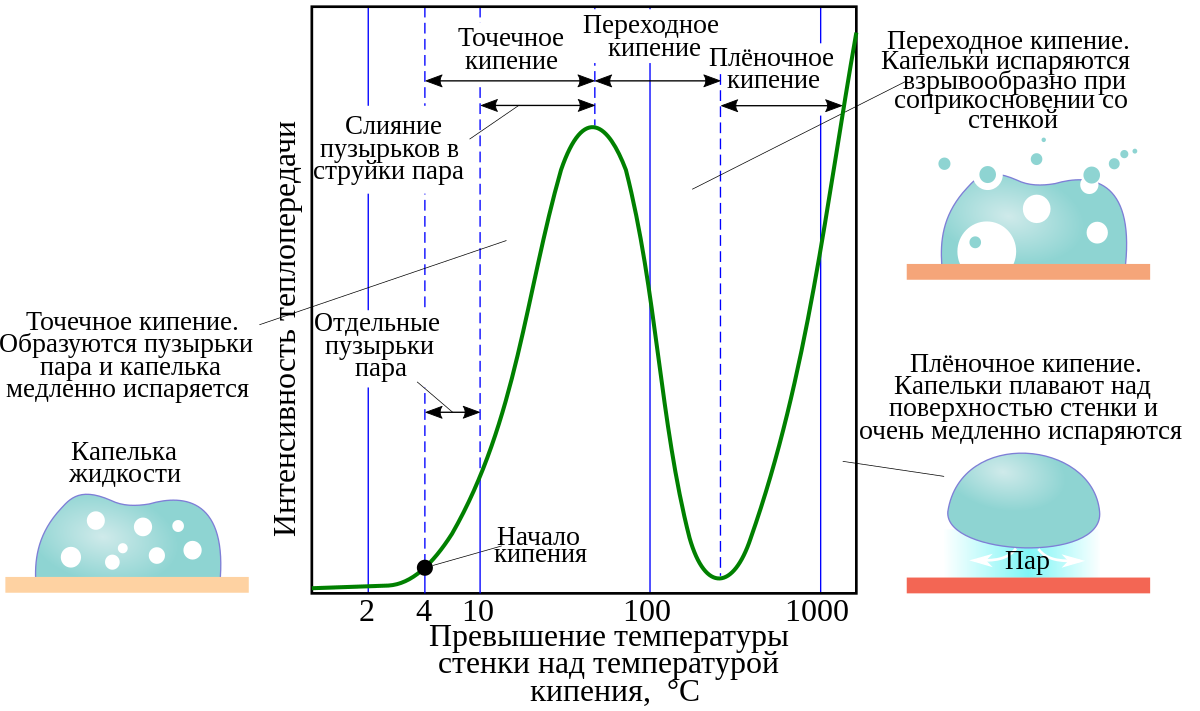
\includegraphics[scale={0.4}]{кипение.png}


\end{center}



\section{Эффект Лейденфроста}

\noindent Явление пленочного кипения капли над горячей поверхностью называется эффектом Лейденфроста. 

\medskip

\noindent Так как теплопроводность пара значительно ниже чем теплопроводность жидкости, при контакте с телом значительно более горячим, чем точка кипения жидкости, создаётся изолирующий слой пара, который предохраняет жидкость от быстрого выкипания.

\medskip

\noindent Основная идея теории такая: с нижней поверхности капли происходит интенсивное испарение, и капля висит на паровой подушке, не касаясь горячей поверхности, аналогично тому, как зависает автомобиль на воздушной подушке. 

\medskip
\begin{center}

\begin{minipage}{.50\textwidth}
  \centering
  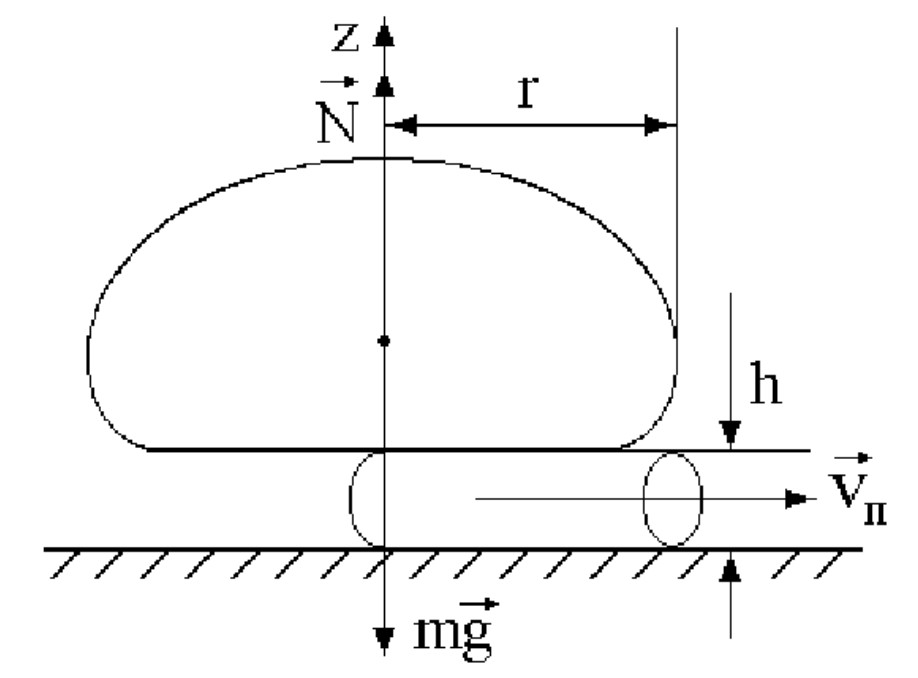
\includegraphics[scale={0.6}]{силы.jpg}
\end{minipage}

\end{center}

\medskip

\noindent Итак, пусть над горячей поверхностью повисла, т.е. находится в состоянии равновесия, капля массой $m$. Равновесие капли как целого означает 

$$N = mg,$$

\noindent где $N$ — сила реакции пара под каплей. Будем наблюдать за равновесием в течение времени, которое гораздо меньше времени испарения всей капли. Тогда приближенно можно считать все величины постоянными. Заметим, что нижняя поверхность капли почти плоская, как и твердая горячая поверхность (это можно пронаблюдать на опыте). Ввиду этого, объем пара под каплей будем считать цилиндрическим, с радиусом $r$ и высотой $h$. 

\medskip

\noindent Пусть избыточное давление пара под каплей равно $\Delta p = p_{\text{п}} - p_{\text{а}}$ ($p_{\text{а}}$ - атмосферное давление). Это давление $\Delta p$ создает в вертикальном направлении силу, уравновешивающую силу тяжести капли, а в горизонтальном направлении — силу, приводящую к вытеканию пара из-под капли со скоростью $v$. Вытеканию препятствует сила трения пара, обусловленная его вязкостью. Тем самым можем записать 

$$ N = \Delta p \pi r^{2} = mg. $$

\noindent Рассмотрим теперь горизонтальные силы. В толще пара мысленно выделим цилиндр с горизонтальной осью длиной $r$ и площадью основания $\Delta S = \frac{1}{4} \pi h^{2}$. Давления на концах цилиндра — $p_{\text{п}}$ и $p_{\text{а}}$. Тогда результирующая сила, действующая на цилиндр, будет равна

$$F_{\text{п}} = (p_{\text{п}} - p_{\text{а}}) \Delta S = \Delta p \Delta S = \Delta p \frac{1}{4} \pi h^{2} .$$

\noindent А по определению силы внутреннего трения в жидкости или газе, она равна
$$F_c = \eta \frac{dv}{dz} \Delta S_\text{бок}, $$
\noindent где $\eta$ — вязкость газа (пара), $\Delta S_{\text{бок}}$ — боковая поверхность горизонтального цилиндра, так как трение осуществляется на ней. Приближенно можно считать

$$\frac{dv}{dz} = \frac{v}{h}$$

\noindent Кроме того, $\Delta S_{\text{бок}} = \pi r h$ ($h$ — диаметр цилиндра, $r$ — его длина). Учитывая силу сопротивления, получим

$$\Delta p = 4 \eta \frac{vr}{{h}^2}. $$

\noindent Исключив перепад давления $\Delta p$, получим следующее выражение для скорости пара:

$$v = \frac{mgh^2}{4 \pi \eta r^3} .$$

\noindent С другой стороны, количество вытекающего пара (а следовательно, и его скорость) определяется скоростью испарения жидкости. Допустим, что в единицу времени к единице площади нижней поверхности капли от горячей поверхности подводится $q$ тепла (удельный тепловой поток). Будем считать, что все это тепло идет на парообразование. Обозначим удельную теплоту парообразования $\lambda$, в единицу времени будет испаряться количество жидкости

$$\Delta m_t = \frac{q \pi r^2}{\lambda}$$

\noindent Если пренебречь обратным процессом конденсации пара, то, по закону сохранения массы, столько же пара выйдет через боковую поверхность цилиндрического парового слоя. Очевидно, через единичную площадку, перпендикулярно ей, в единицу времени проходит количество пара, равное $\rho_{\text{п}} v$ ($\rho_{\text{п}}$ — плотность пара). Тогда через всю боковую поверхность парового слоя $S = 2 \pi \rho h$ за секунду пройдет количество пара

$$ \Delta m_t = \rho_{\text{п}} v \cdot 2 \pi \rho h . $$

\noindent Найдем связь удельного теплового потока и скорости истечения пара:

$$ v = \frac{qr}{2 \lambda \rho_{\text{п}}} h . $$

\noindent Найдем величину удельного теплового потока, который необходимо подвести к капле, чтобы она висела на паровой подушке: 

$$ q = \frac{mg \lambda \rho_{\text{п}} h^3}{2 \pi r^4 \eta} . $$

\noindent Зная тепловой поток, нетрудно найти температуру поверхности, при которой возможно явление Лейденфроста. Как известно, удельный тепловой поток связан с перепадом температур соотношением

$$ q_z = - \varkappa \frac{\partial T}{\partial z} ,$$

\noindent где $\varkappa$ — коэффициент теплопроводности среды (пара), а знак «—» говорит о том, что тепло распространяется в сторону уменьшения температуры. В нашем случае можно приближенно записать

$$ q = \varkappa \frac{\partial {(T_{\text{л}} - T_{\text{к}}})}{\partial h}  $$

Тогда

$$ T_{\text{л}} = T_{\text{к}} + \frac{mg \lambda \rho_{\text{п}} h^4 }{2 \pi r^4 \eta \varkappa} ,  $$

\noindent где $T_{\text{к}}$ — температура нижней поверхности капли, которую можно принять равной $\approx$ 100°С.
\noindent Итак, $m$ и $r$ легко если и не измерить, то оценить из опыта, а $\lambda, \rho_{\text{п}}, \eta, \varkappa$ можно найти в таблицах.

\medskip

\noindent Измерим на опыте $T_{\text{л}}$, при которой становится возможным явление Лейденфроста, и по формуле найдем толщину прослойки пара $h$.

\medskip

\noindent Для экспериментального определения $T_{\text{л}}$ будем использовать газовую плиту, алюминиевую кастрюлю, мультиметр с термопарой (предел измерения температуры 400°С), шприц и секундомер. 

\medskip
\begin{center}


  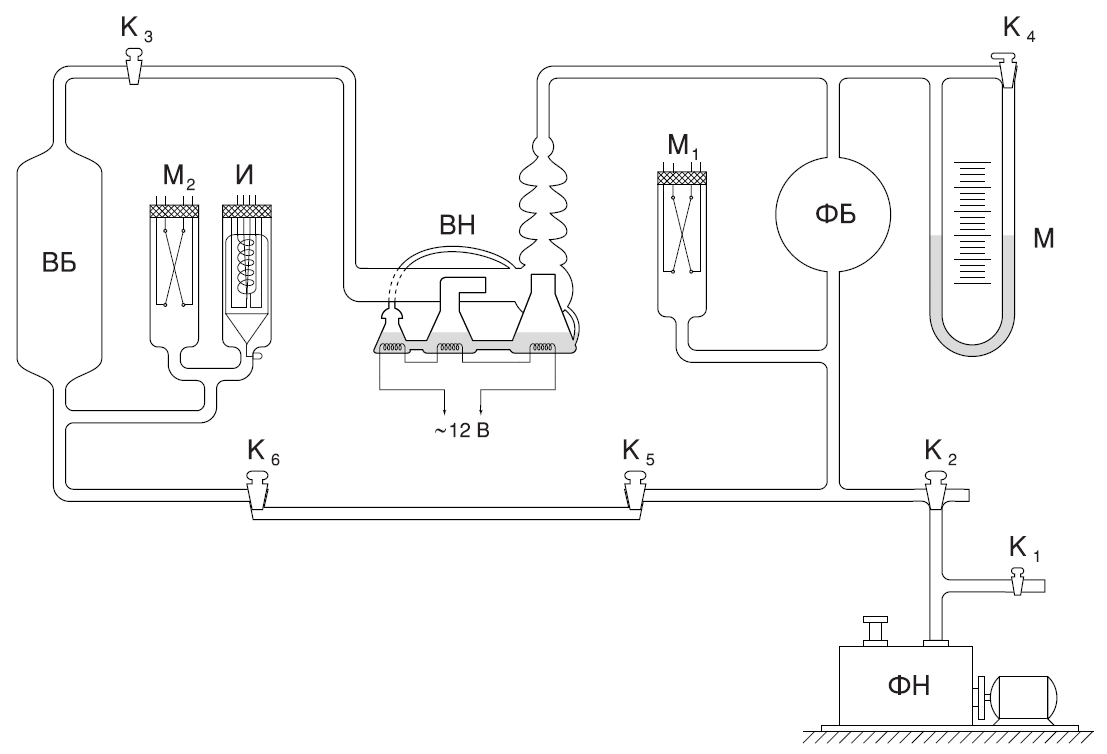
\includegraphics[scale={0.32}]{установка.png}


\end{center}

\medskip

\noindent По результатам измерений построим график зависимости времени жизни капли от температуры поверхности.



\begin{center}
  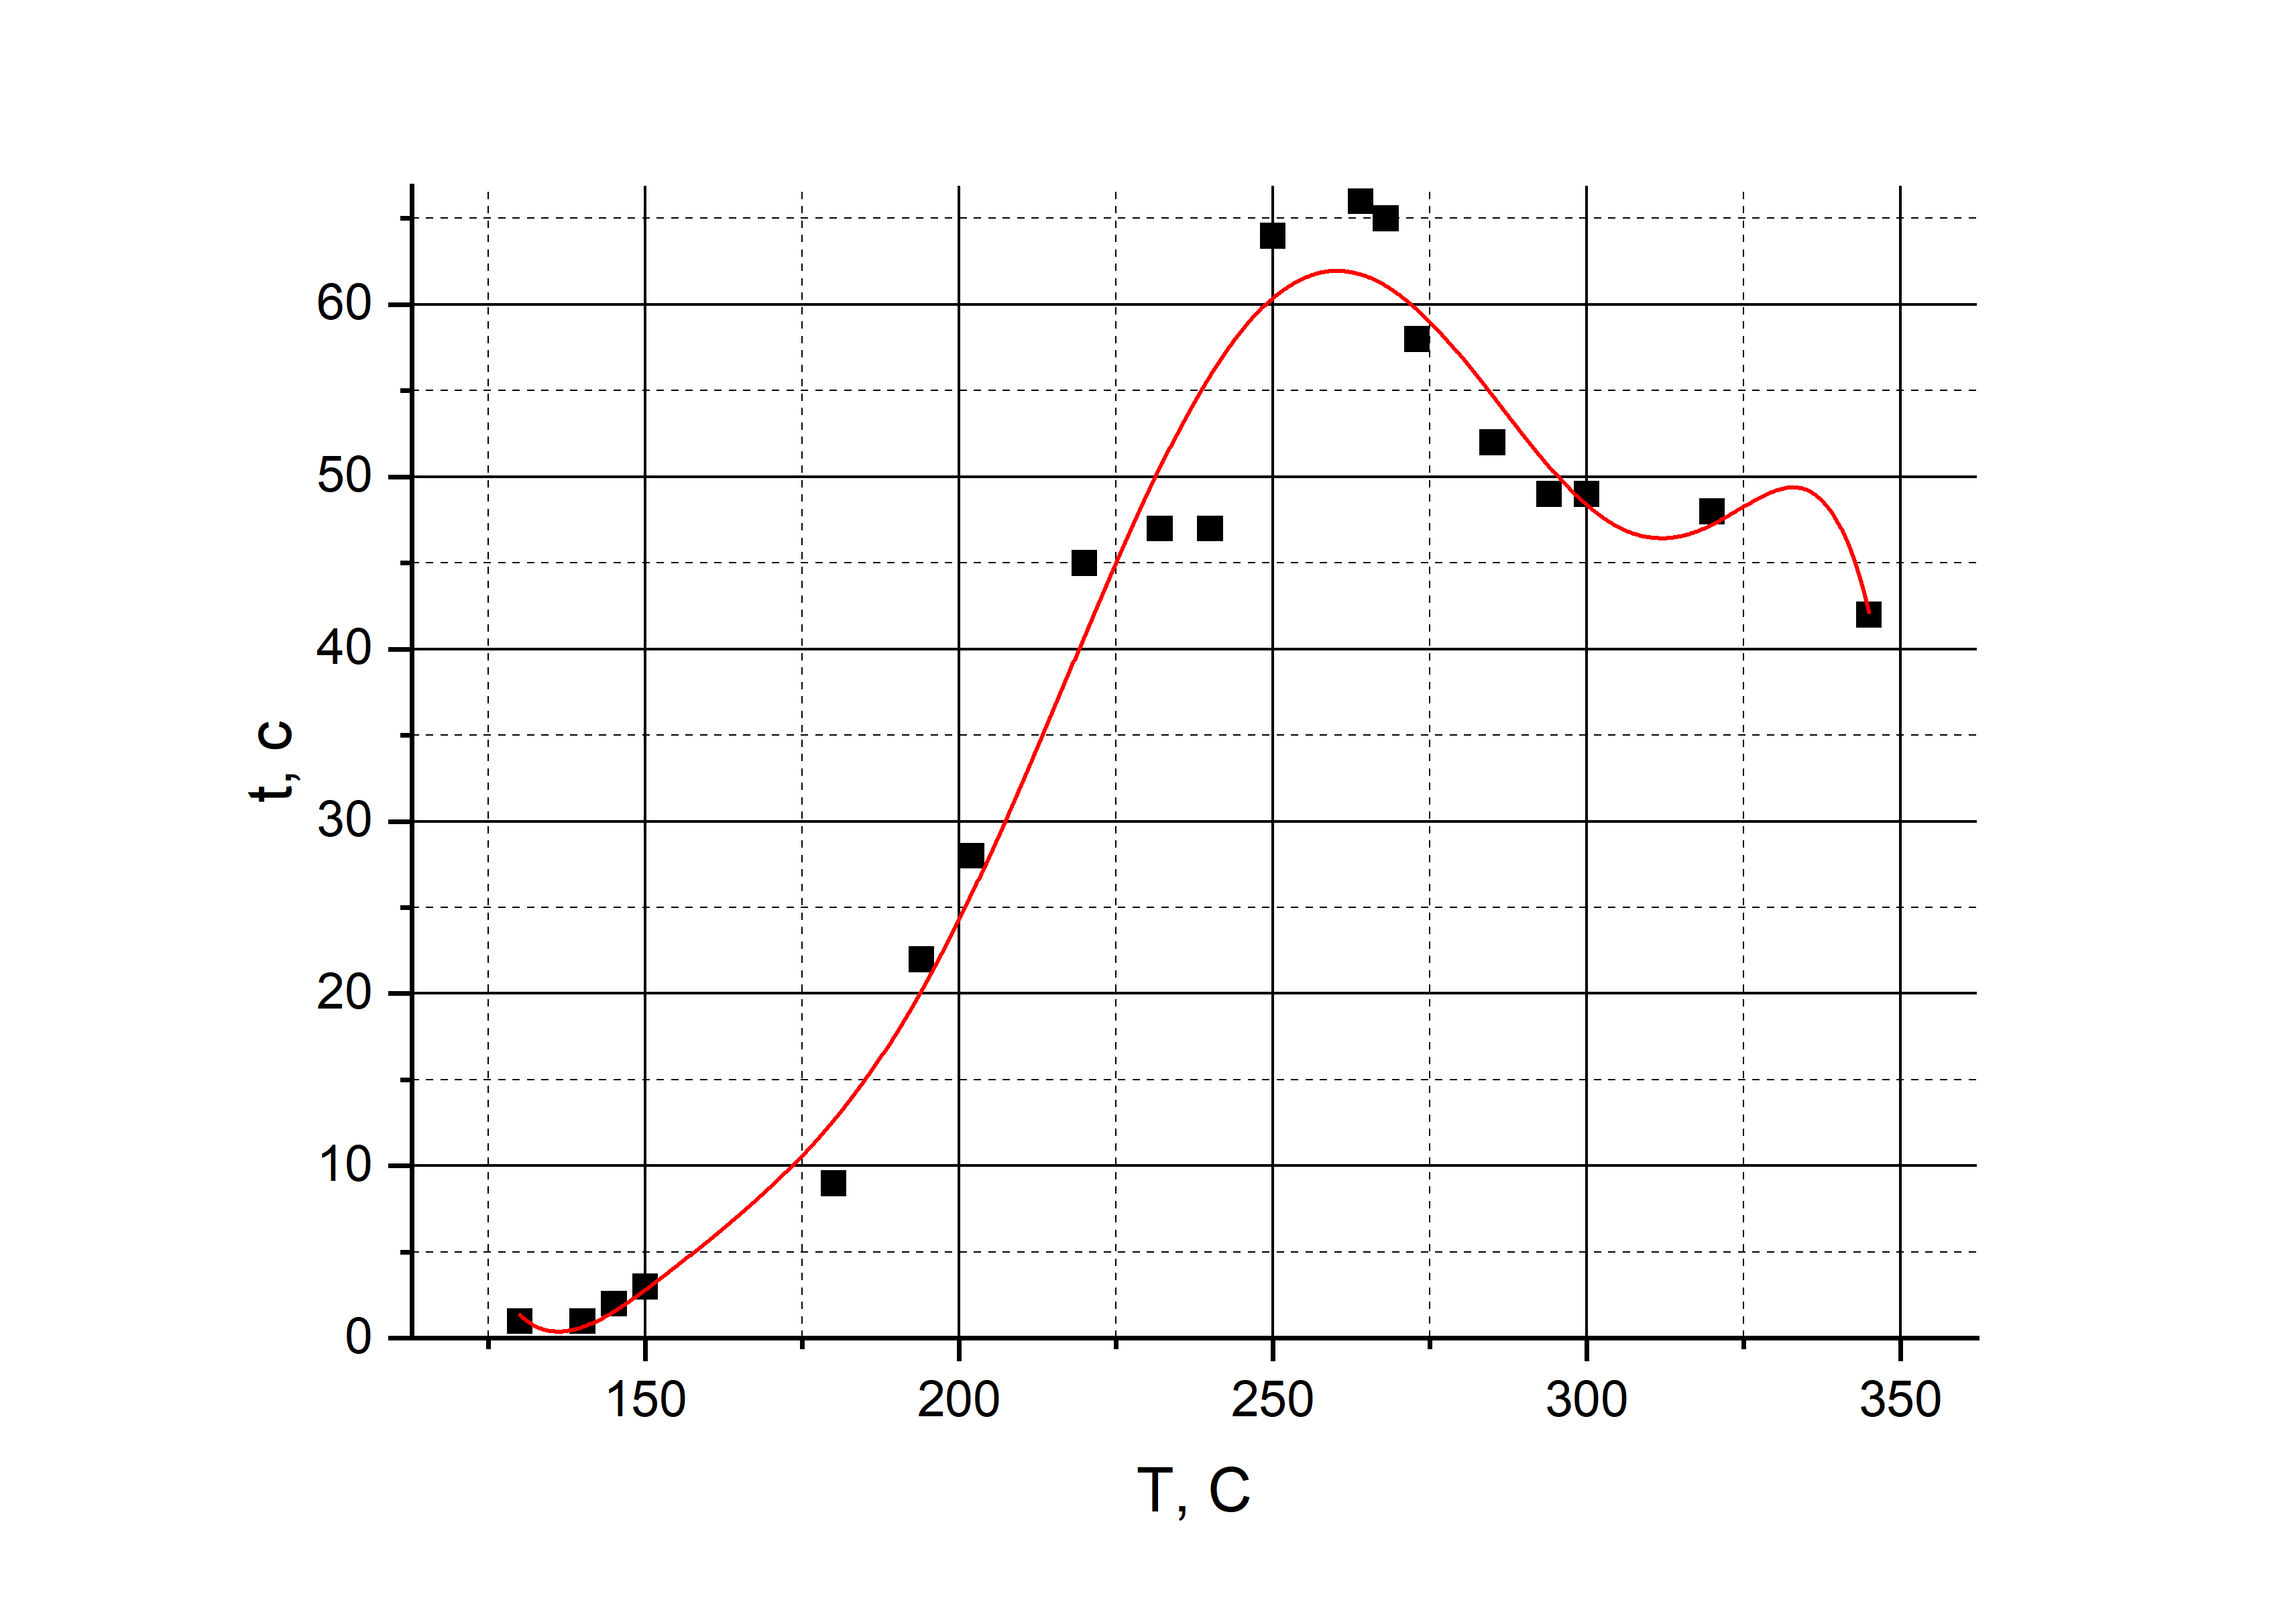
\includegraphics[scale={0.6}]{график.png}
\end{center}


\medskip

\noindent Из графика $T_{\text{л}} \approx 270$°С.

\medskip

\noindent Оценим параметры капли:

$$ r \approx 3 \text{ мм}$$

$$ m \approx 1,13 \cdot 10^{-4} \text{ кг}$$

\noindent Табличные данные:

$$ \lambda = 2,3 \cdot 10^6 \frac{\text{Дж}}{\text{кг}}\text{, } \eta = 1,7 \cdot 10^{-5} \text{ Па} \cdot \text{с}\text{, } \rho_{\text{п}} = 0,6 \frac{\text{кг}}{\text{м}^3}\text{, } \varkappa = 2,4 \cdot 10^{-2} \frac{\text{Вт}}{\text{м К}} $$

\noindent Тогда $h \approx 9 \cdot 10^{-5} \text{ м} = 0,09 \text{ мм}$.


\medskip

\section{Колебания капли}

\noindent Как и всякая система в равновесии, капля может совершать колебания около положения равновесия. Для сферического равновесия может быть решена задача об определении форм собственных колебаний капли. На рисунке показано несколько форм колебаний капли (их называют модами). Моды нумеруются. Первой модой (n = 1) колебаний сферы являются чисто радиальные колебания, соответствующие одинаковому во всех точках сферы увеличению (уменьшению) радиуса. Возможных мод колебаний бесконечно много. Реальное колебание представляет собой совокупность различных мод, но наблюдатель обычно видит одну доминирующую моду, которой соответствует наибольшая амплитуда. Например, наиболее часто можно увидеть вторую моду n = 2, но можно пронаблюдать на опыте и 5—6 первых мод. 
\medskip



\begin{center}
  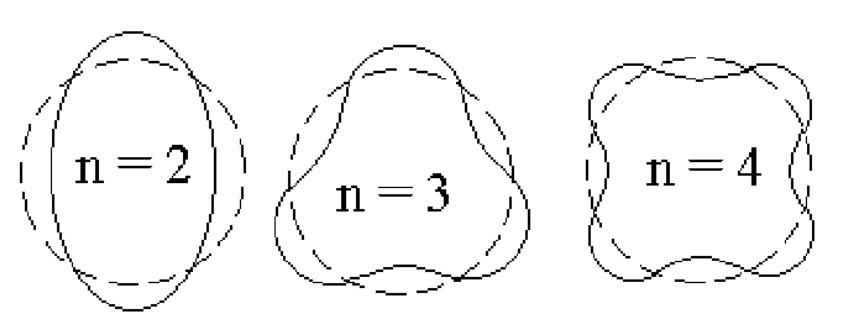
\includegraphics[scale={0.7}]{моды.jpg}
\end{center}

\medskip

\noindent Оценим частоту колебаний основной моды теоретически и экспериментально.

\medskip

\noindent Оценку частоты колебаний капли можно произвести, используя теорию размерностей. Очевидно, что частота колебаний может зависеть только от плотности жидкости $\rho$, коэффициента поверхностного натяжения $\sigma$, радиуса капли $r$. Тогда можно описать с точностью до постоянного множителя
$$\omega \approx \rho^m \sigma^n r^k . $$
\noindent Размерность правой части получается следующей:
$$ {\text{кг}}^{n+m} {\text{м}}^{k-3m} {\text{с}}^{-2n} . $$
\noindent Размерность левой - ${\text{с}}^{-1}$ . Приравнивая размерности, получим:
\begin{equation*}
 \begin{cases}
   -2n = -1\text,\qquad \qquad n = 1/2,\\
   n + m = 0 \text,\qquad \qquad m = -1/2,\\
   k - 3m = 0 \text,\qquad \qquad k = -3/2.
 \end{cases}
\end{equation*}

\noindent Получаем
$$\omega \sim \sqrt{\frac{\sigma}{\rho r^3}} .$$

\medskip

\noindent Точный результат для второй моды n = 2 таков:
$$\omega = \sqrt{\frac{8 \sigma}{\rho r^3}} .$$

\noindent Тогда теоретическая оценка частоты колебаний: 

$$ \omega = \sqrt{\frac{8 \cdot 71,7 \cdot 10^{-3}}{10^3 \cdot (5 \cdot 10^{-3})^3}} = 4,8 \text{ Гц} $$

\medskip

\noindent Оценим экспериментально частоту колебаний капли для n = 2.

$$ \omega \approx 4,3 \text{ Гц}. $$


\begin{center}
  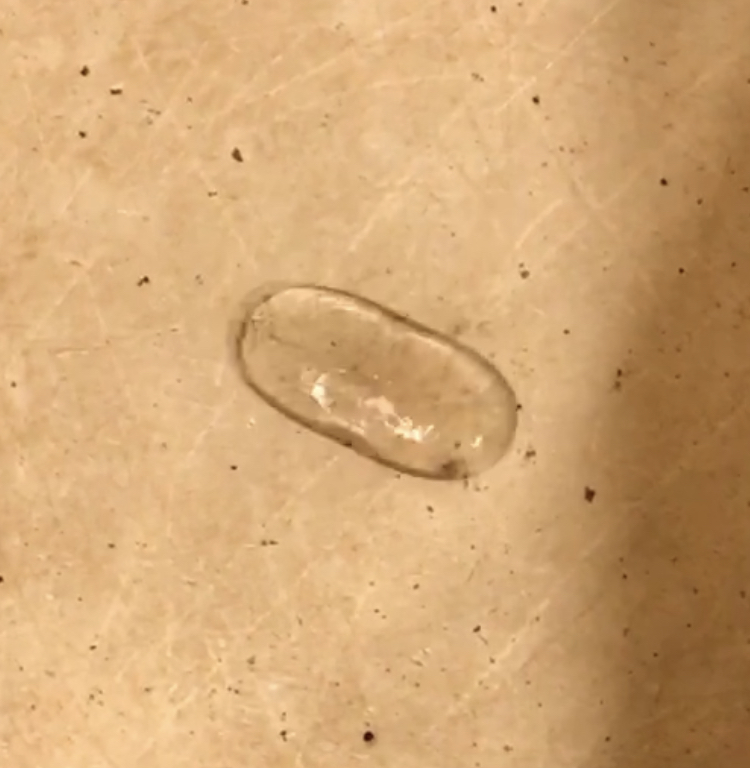
\includegraphics[scale={0.2}]{капля.png}
\end{center}


\medskip

\noindent Экспериментальные данные с хорошей точностью соотносятся с теоретическими.





\section{Список использованной литературы}

\noindent Саранин В.А. Равновесие жидкостей и его устойчивость. Простая теория и доступные опыты.–М.:Институт компьютерных исследований, 2002.–144с

\medskip

\noindent Голубев М., Кагаленко А. Капля на горячей поверхности // Квант.–1977.–№12.– С.28-19.

\medskip

\noindent Лушков А., Лужков Ю. «Звезды» из водяной капли // Квант.–1978.–№7.– С.28.


\medskip

\noindent Уокер Дж. Как кипит вода? (Эффект Лейденфроста) // Квант.–1991.–№6.– С.33-35.

\end{document}